\documentclass[a4paper]{article}

\usepackage[english]{babel}
\usepackage[utf8]{inputenc}
\usepackage{amsmath}
\usepackage{graphicx}
\usepackage[colorinlistoftodos]{todonotes}
\usepackage{pdfpages}

\title{Concepts Avancés de Bases de données}

\author{Joaquim LEFRANC et Jérôme Skoda}

\date{\today}

\begin{document}
\maketitle


\section{Nouveauté depuis le TP3}

\begin{itemize}
	\item 6 test en plus (table de hash + hash join)
	\item 1 demo (make demo-tp4)
	\item Nouvelle structure de donnée hashtable (réutilisable et encapsulé)
\end{itemize}

\section{Comment compiler le projet}

\subsection{Avec le terminal}

\begin{itemize}
	\item make all : Compile tout les fichiers
	\item make test : Lancement de la série de tests automatiques
	\item make doc  : Génération de la documentation (doxygen)
	\item make rapport : Génération du rapport (latex)
	\item make clean : Nettoyage du projet (supression des objets et binaires)
	\item make demo-tp1 : Lancer la démo tp1
	\item make demo-tp2 : Lancer la démo tp2
	\item make demo-tp3 : Lancer la démo tp3
	\item make demo-tp4 : Lancer la démo tp4 (Nouveau)
	\item make rm-rs : Supprime le fichier res/RS.txt
\end{itemize}

\subsection{Avec ECLIPSE}

Pour lancer une commande utiliser les builds targets.

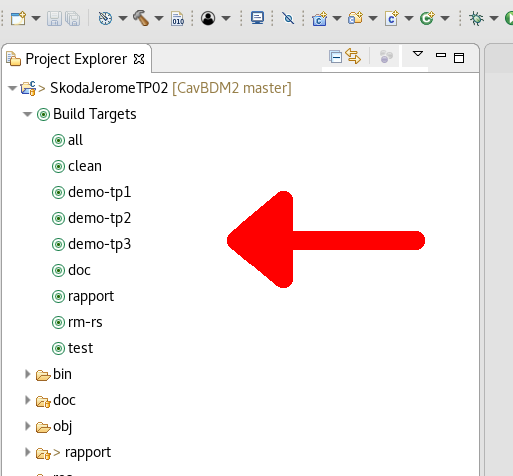
\includegraphics[width=0.5\textwidth]{builds-target.png}

\section{Arborescence}

\begin{itemize}
\item bin : Binaire exécutable
\begin{itemize}
  \item demo : Exécutable de démonstration
  \item test : Exécutable de test
\end{itemize}
\item doc : Documentation doxygen sous differents formats
\item rapport : Source du rapport
\item res : Ressources necessaire au projet (fichier de bdd)
\item script  : Script utilisé pour les test
\item src : Source du projet
\begin{itemize}
  \item bdd   : Source de la bibliothéque
  \item demo  : Sources des differentes démonstrations d'utilisation
  \item test  : Sources des dufferents tests
\end{itemize}

\item sujet.pdf  : Sujet du projet
\item README.md  : Le readme du projet 
\item rappot.pdf : C'est moi
\item refman.pdf : Documentation format pdf
\end{itemize}

\section{Caracteristiques}

\begin{itemize}
	\item Le code est organisé
	\item Il y a des code des tests
	\item Il y a la doc
	\item Il y a un rapport
	\item Et il y a pleins d'autre chose
\end{itemize}

\section{Démonstration}

Les sources de demosntration sont diponible dans: src/demo
Les exécutables de test sont généré dans: bin/demo
La commande make pour lancer les demo sont: make demo-tp1, make demo-tp2, make demo-tp3 etc...

\begin{itemize}
  \item tp1-natural-join: Natural join R et S
  \item tp2-merge-join-without-duplicate: Merge join sans duplication 
  \item tp3-merge-join-with-duplicate: Merge join avec duplication 
  \item tp4-hash-join : Hash join (Nouveau)
\end{itemize}

\section{Test unitaire}

Les sources de test sont diponible dans: src/test
Les exécutables de test sont généré dans: bin/test
Le script de test est dans script/test.sh
La commande make pour lancer les test est: make test

\begin{itemize}
  \item 00-storeFileBuffer: Ecriture d'un buffer dans un fichier
  \item 01-natural-join-1: Natural join R et S
  \item 02-natural-join-2: Natural join S et R
  \item 03-buf-quick-sort: Fonction de trie d'un buffer
  \item 04-merge-join-without-duplicate-1: Merge join sans duplication R et S
  \item 05-merge-join-without-duplicate-2: Merge join sans duplication S et R
  \item 06-merge-join-with-duplicate-1: Merge join avec duplication R et S
  \item 07-merge-join-with-duplicate-2: Merge join avec duplication S et R
  \item 08-hash-put-equilibre : Test ajout equilibré dans une table de hash (Nouveau)
  \item 09-hash-put-desequilibre : Test ajout déséquilibré dans une table de hash (Nouveau)
  \item 10-hash-full : Test remplissage complet dans une table de hash (Nouveau)
  \item 11-hash-get : Test recupreration d'une entrée dans la table de hash (Nouveau)
  \item 12-hash-remove : Test supression / rehash dans une table de hash (Nouveau)
  \item 13-hash-join : Test hash join (Nouveau)
\end{itemize}

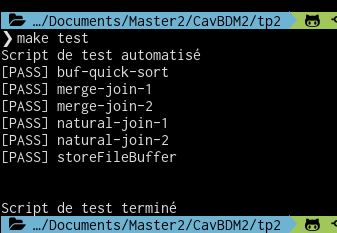
\includegraphics[width=0.8\textwidth]{test.png}

\end{document}
              
